\documentclass[12pt, letterpaper]{article}
\usepackage[mmddyyyy]{datetime}

\usepackage[utf8]{inputenc}
\usepackage{amsmath}
\usepackage{mathpazo}
\usepackage{mathtools}
\usepackage{eulervm}
\usepackage[skip=10pt plus1pt]{parskip}
\usepackage{textalpha}

\usepackage[margin=1in]{geometry}
\linespread{1.20}
\usepackage{enumerate}
\usepackage{enumitem}
\usepackage{listings}
\usepackage[T1]{fontenc}
\usepackage{amsfonts}
\usepackage{amssymb}
\usepackage{amsthm}
\usepackage{multirow,array}
\usepackage{graphicx}
\usepackage{physics}
\usepackage{bm}
\usepackage{tikz}
\usepackage[longnamesfirst]{natbib}
\usepackage{comment}
\usepackage{setspace}
\usepackage{hyperref}
\usepackage{accents}
\usepackage{graphicx}
\usepackage{float}
\usepackage{fancyvrb}
\usepackage{cancel}

\VerbatimFootnotes

\graphicspath{{Images/}}
\setlength{\parindent}{0pt}

\newtheorem{theorem}{Theorem}
\newtheorem{corollary}{Corollary}
\newtheorem{lemma}{Lemma}
\newtheorem{definition}{Definition}
\newtheorem{axiom}{Axiom}
\newcommand{\e}{\mathrm{e}}
\newcommand{\Var}{\mathrm{Var}}
\newcommand{\Ex}[1]{\mathbb{E}\left[#1\right]}
\renewcommand{\Pr}[1]{\mathbb{P}(#1)}
\newcommand{\plim}{\mathrm{plim}}
\newcommand{\pc}[1]{\frac{\dot{#1}(t)}{#1(t)}}
\renewcommand\qedsymbol{$\blacksquare$}
\newcommand{\ubar}[1]{\underaccent{\bar}{#1}}

\title{Homework 14 \\Actuarial Corporate Finance}
\author{Alejandro Flores-Brown}

\begin{document}

    \maketitle

    Note: I have passed Exam FAM (through the exam process, not UEC), which required me to learn much of the material in this section. My notes may be comparatively sparse accordingly.

    \section{Notes}

    \subsection{Video 15a}

    Call option: right to purchase an asset from a seller at a fixed \emph{strike price} \(K\) at a given time \(T\). This gives a return structure of \(S_T - K\) when \(S_T > K\) and \(0\) when \(S_T < K\) -- in the former case, the owner of the option exercises it and gets an asset worth \(S_T\) for only \(K\), while in the latter case exercising the option would lose money so it is not exercised. Taking the price as the \emph{option premium} \(\pi > 0\),  this gives the buyer a payout of 

    \[ \max \left\{S_T - K, 0\right\}   \]

    and a profit of

    \[ \pi = \max \left\{ S_T - K, 0 \right\} - \pi \e^{rT}    \]

    (The seller has payoff and profit functions that are the negative of the buyers').

    Now we examine an exercise. We are given a call option on a share of stock with strike price 100 and expiration date 12/31/2016.

    \begin{enumerate}
    
        \item We will exercise the option if the stock price is greater than the strike price at the expiration date, which means that \(S_T > 100\) at the end of \(2016\).
        \item If the stock price is \(120\), we will exercise the option, giving the seller the strike price \(100\) and receiving a share of stock worth \(120\) (or just the cash value, in practice!). This gives a net payoff of \(120 - 100 = 20\).
        \item Now we suppose the stock price is \(90\) at the end of \(2016\). In this case we do not exercise the option, so no transaction takes place and we have a payoff of \(0\).  
        \item The revenue function is \(\max\left\{S_T - 100, 0\right\}\). It is graphed below. 
        \begin{figure}[H]
	    \centering
	    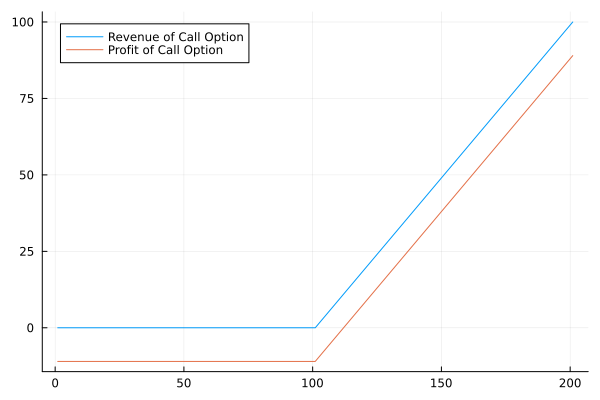
\includegraphics[scale=0.7]{rev_prof_plot_1.png}
	    \end{figure}
        Code:
        \begin{verbatim}
using Plots
rev = max.(range(0.0, 200.0, 201) .- 100, 0)
profit = rev .- 10*(1 + 0.1)
plot_rp = plot([rev profit], 
            label=["Revenue of Option" "Profit of Option"])
png(plot_rp, "rev_prof_plot_1")
        \end{verbatim}
        \item The profit function is \(\max\left\{S_T - 100, 0\right\} - 10 \times (1 + 0.1)\). It is graphed with the revenue function above.
        \item Why would we buy this option? Maybe we believe that the stock has a better outlook than the market predicts via the price over the lifespan of the option. The option provides a convenient way to profit off of this belief (provided we are correct) that also gives limited exposure to losses if the stock price drops.

    \end{enumerate}

    \subsection{Video 15b}

    The call option lets a buyer buy an asset for a fixed price; the \emph{put option} lets the owner sell an asset for a fixed price \(K\) at time \(T\). As before, this is an option, so you are not forced to sell; therefore, the option will only be exercised if \(S_T < K\). This gives a payoff of 
    
    \[ \max\left\{K - S_T, 0\right\}    \]

    and profit

    \[ \max\left\{K - S_T, 0\right\} - \pi \e^{rT}   \]

    for the buyer. (The seller has payoff and profit functions that are the negative of the buyers').

    Now we examine an exercise. We are given a put option on a share of stock with strike price \(100\) and expiration date 12/31/2016 -- effectively the previous problem mutatis mutandis.

    \begin{enumerate}
    \item We will exercise the option if the stock price is less than the strike price \(100\) at time \(T\).
    \item  If \(S_T = 120 > K\), then we do not exercise the option. There is no transaction, the option expires, and the net payoff is \(0\).
    \item Now the stock price is \(90 < K = 100\) so we do exercise the option. We sell one share of the stock, or \(90\), to the buyer, and receive \(100\) in cash. This gives a net payoff of \(10\)
    \item With a very similar code to before, we construct the revenue and profit graphs. The revenue function is \(\max\left\{100 - S_t, 0\right\}\)
    \begin{figure}[H]
	    \centering
	    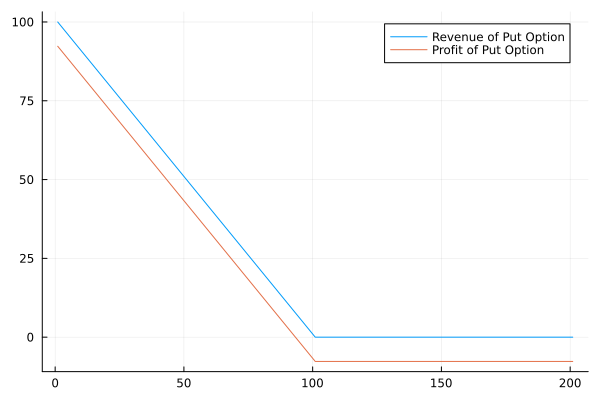
\includegraphics[scale=0.7]{rev_prof_plot_2.png}
	\end{figure}
    Code:
    \begin{verbatim}
using Plots
rev2 = max.(100.0 .- (range(0.0, 200.0, 201)), 0)
profit2 = rev2 .- 7*(1 + 0.1)
plot_rp2 = plot([rev2 profit2], 
            label=["Revenue of Put Option" "Profit of Put Option"])
png(plot_rp2, "rev_prof_plot_2")
    \end{verbatim}
    \item The profit function is \(\max\left\{100 - S_T, 0\right\} - 7 \times (1 + 0.1)\). It is graphed with the revenue function above.
    \item The put option pays off if the company's stock loses value, so the put is effectively a bet against the market's valuation of the company. You sell the put if you believe the market's stock price is incorporating an unwarranted positive evaluation of the company's prospects.
    \end{enumerate}



    \subsection{Video 15c}

    We start with another exercise. We are given \(T = 2\), \(\pi = 8.52\), and \(r = 0.048\). The profit given a spot price of \(85\) at expiration is \(2.36\). We need to find \(K\). To answer this question we need to write the profit function:

    \[ \text{profit} = 8.52 \times 1.048^2 - \max\left\{K - 85,0\right\} = 2.36   \]

    Clearly for us to have positive profit, we need to have \(K > S_T\). That gives us

    \[ 8.52 \times 1.048^2 - 2.36 \approx 7 = K - 85 \implies K = 92       \]

    Now we return to notes. There is a concept associated with options called \emph{moneyness}: an option is at-the-money if the spot price equals the strike price, in-the-money if exercising the option is preferable at current values (i.e. given current stock price, interest rates, etc.), and out-of-the-money if exercising the option would not be preferable at current values. We also should know something about the terminology associated with options: \emph{European} options can only be exercised at an expiration date \(T\), \emph{American} options can be exercised at any time until \(T\), and Bermudan options can only be exercised at maturity or during a specially declared time period. (We will only think about European options in this module, or on the related Exam FAM.)

    \section{H 14-1}

    We are given a stock with a current price of \(S_0 = 11\), an option with a strike price of \(S_T = 9\) and a cost of \(\pi = 2.8\), a final price of \(K = 5\), a duration of \(T = 0.5\) years, and a continuous risk-free rate of \(r = 0.045\). However, much of this information is not necessary! We see that the final price \(S_T\) is less than the strike price, so we choose not to exercise our options. That means our final loss is just what we paid to buy the options:

    \[ 100 \left( 0 - 2.8 \e^{0.5 \times 0.045} \right) = -273.77  \]

    \section{H 14-2}

    Given that the short position's payoffs and profit of the call and put are the negatives of the long position's, I assume this will also hold for stocks and bonds.

    \subsection{}

    \begin{figure}[H]
	    \centering
	    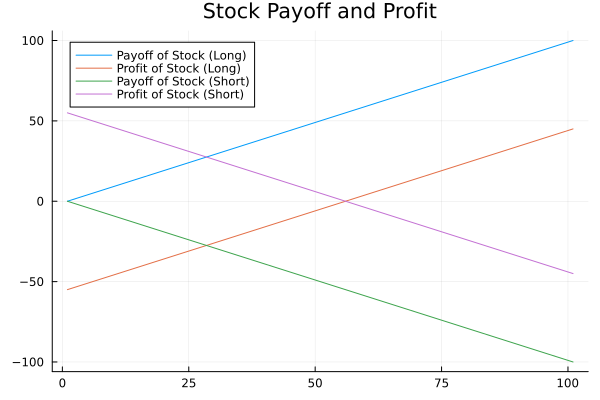
\includegraphics[scale=0.4]{stock_plot.png}
	\end{figure}

    \subsection{}

    \begin{figure}[H]
	    \centering
	    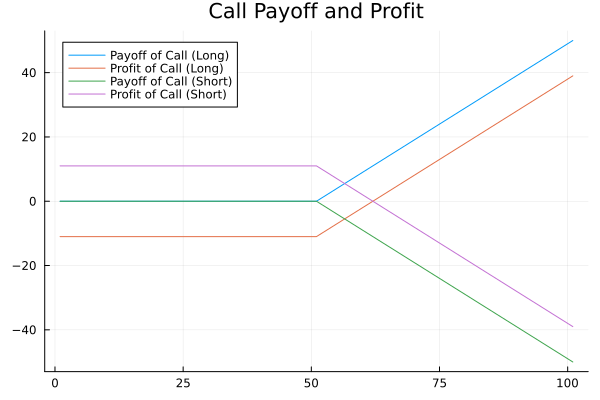
\includegraphics[scale=0.4]{call_plot.png}
	\end{figure}

    \subsection{}

    \begin{figure}[H]
	    \centering
	    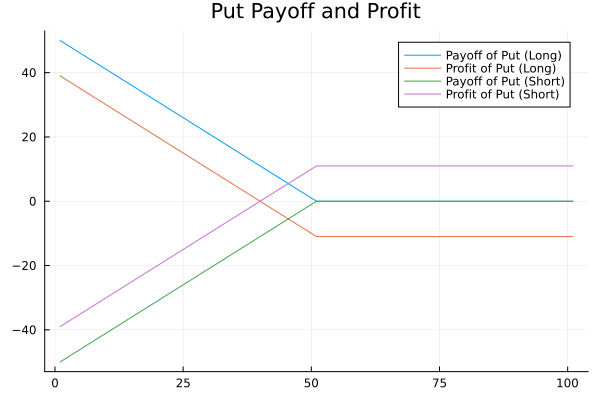
\includegraphics[scale=0.4]{put_plot.png}
	\end{figure}

    \subsection{}

    \begin{figure}[H]
	    \centering
	    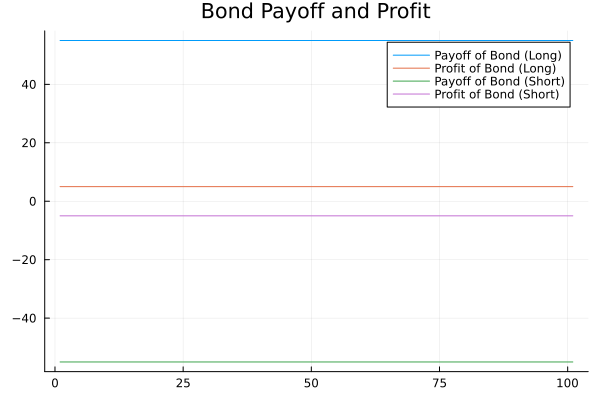
\includegraphics[scale=0.4]{bond_plot.png}
	\end{figure}

    Code (numbers are chosen for illustrative purposes and are not equilibrium values):

    \begin{verbatim}
    brange = range(0.0, 100.0, 101)
S_0 = 50.0
price_option = 10.0
R = 1.1

payoff_stock = brange
profit_stock = payoff_stock .- S_0*R

sh_payoff_stock = -1*payoff_stock
sh_profit_stock = -1*profit_stock

payoff_call = max.(brange .- S_0, 0.0)
payoff_put = max.(S_0 .- brange, 0.0)
sh_payoff_call = -1*payoff_call
sh_payoff_put = -1*payoff_put

profit_call = payoff_call .- price_option*R
profit_put = payoff_put .- price_option*R 
sh_profit_call = -1*profit_call 
sh_profit_put = -1*profit_put 

price_bond = 50.0
payoff_bond = (price_bond*R).*ones(length(brange))
profit_bond = (price_bond*(R - 1.0)).*ones(length(brange))
sh_payoff_bond = -1*payoff_bond
sh_profit_bond = -1*profit_bond


stock_plot = plot([payoff_stock profit_stock sh_payoff_stock sh_profit_stock], 
title = "Stock Payoff and Profit", 
labels = ["Payoff of Stock (Long)" "Profit of Stock (Long)" 
"Payoff of Stock (Short)" "Profit of Stock (Short)"])
call_plot = plot([payoff_call profit_call sh_payoff_call sh_profit_call], 
title = "Call Payoff and Profit", 
labels = ["Payoff of Call (Long)" "Profit of Call (Long)" 
"Payoff of Call (Short)" "Profit of Call (Short)"])
put_plot = plot([payoff_put profit_put sh_payoff_put sh_profit_put], 
title = "Put Payoff and Profit", 
labels = ["Payoff of Put (Long)" "Profit of Put (Long)" 
"Payoff of Put (Short)" "Profit of Put (Short)"])
bond_plot = plot([payoff_bond profit_bond sh_payoff_bond sh_profit_bond], 
title = "Bond Payoff and Profit", 
labels = ["Payoff of Bond (Long)" "Profit of Bond (Long)" 
"Payoff of Bond (Short)" "Profit of Bond (Short)"])

png(stock_plot, "stock_plot")
png(call_plot, "call_plot")
png(put_plot, "put_plot")
png(bond_plot, "bond_plot")
    \end{verbatim}

\end{document}